% This is "aamas2016_sample.tex", a revised version of aamas2015_sample.tex
% This file should be compiled with "aamas2016.cls"
% This example file demonstrates the use of the 'aamas2015.cls'
% LaTeX2e document class file. It is intended for those submitting
% articles to the AAMAS-2016 conference. This file is based on
% the sig-alternate.tex example file.
% The 'sig-alternate.cls' file of ACM will produce a similar-looking,
% albeit, 'tighter' paper resulting in, invariably, fewer pages
% than the original ACM style.
%
% ----------------------------------------------------------------------------------------------------------------
% This .tex file (and associated .cls ) produces:
%       1) The Permission Statement
%       2) The Conference (location) Info information
%       3) The Copyright Line with AAMAS data
%       4) NO page numbers
%
% as against the acm_proc_article-sp.cls file which
% DOES NOT produce 1) through 3) above.
%
% Using 'aamas2015.cls' you don't have control
% from within the source .tex file, over both the CopyrightYear
% (defaulted to 20XX) and the IFAAMAS Copyright Data
% (defaulted to X-XXXXX-XX-X/XX/XX).
% These information will be overwritten by fixed AAMAS 2015  information
% in the style files - it is NOT as you are used to with ACM style files.
%
% ---------------------------------------------------------------------------------------------------------------
% This .tex source is an example which *does* use
% the .bib file (from which the .bbl file is produced).
% REMEMBER HOWEVER: After having produced the .bbl file,
% and prior to final submission, you *NEED* to 'insert'
% your .bbl file into your source .tex file so as to provide
% ONE 'self-contained' source file.
%


%\documentclass{aamas2016}
\documentclass{aamas2016_extendedabstract}

\usepackage{tikz}
\usetikzlibrary{arrows,positioning,automata}
\usepackage[noend]{algpseudocode}
\usepackage{algorithm}
\usepackage{enumitem, kantlipsum}

% if you are using PDF LaTeX and you cannot find a way for producing
% letter, the following explicit settings may help

\pdfpagewidth=8.5truein
\pdfpageheight=11truein

\begin{document}

% In the original styles from ACM, you would have needed to
% add meta-info here. This is not necessary for AAMAS 2015  as
% the complete copyright information is generated by the cls-files.


\title{Expectedness in Human-Robot Collaboration}

% AUTHORS


% For initial submission, do not give author names, but the
% tracking number, instead, as the review process is blind.

% You need the command \numberofauthors to handle the 'placement
% and alignment' of the authors beneath the title.
%
% For aesthetic reasons, we recommend 'three authors at a time'
% i.e. three 'name/affiliation blocks' be placed beneath the title.
%
% NOTE: You are NOT restricted in how many 'rows' of
% "name/affiliations" may appear. We just ask that you restrict
% the number of 'columns' to three.
%
% Because of the available 'opening page real-estate'
% we ask you to refrain from putting more than six authors
% (two rows with three columns) beneath the article title.
% More than six makes the first-page appear very cluttered indeed.
%
% Use the \alignauthor commands to handle the names
% and affiliations for an 'aesthetic maximum' of six authors.
% Add names, affiliations, addresses for
% the seventh etc. author(s) as the argument for the
% \additionalauthors command.
% These 'additional authors' will be output/set for you
% without further effort on your part as the last section in
% the body of your article BEFORE References or any Appendices.

%\numberofauthors{8} %  in this sample file, there are a *total*
% of EIGHT authors. SIX appear on the 'first-page' (for formatting
% reasons) and the remaining two appear in the \additionalauthors section.
%

\numberofauthors{3}

\author{
Mahni Shayganfar, Charles Rich, Candace L. Sidner\\
       \affaddr{Worcester Polytechnic Institute}\\
       \affaddr{100 Institute Road}\\
       \affaddr{Worcester, Massachusetts}\\
       \email{mshayganfar, rich, sidner@wpi.edu}
}

\maketitle

\begin{abstract}
We have investigated the mutual influences of affective and collaborative
processes in a cognitive theory to support interaction between humans and robots
or virtual agents. We build primarily on the \textit{cognitive appraisal} theory of
emotions and the \textit{SharedPlans} theory of collaboration to investigate the
structure, fundamental processes and functions of emotions in a collaboration.
We have developed new algorithms for appraisal processes as part of a new
overall computational model. In this paper, we provide the \textit{expectedness}
appraisal algorithm for collaboration context. We have evaluated our implemented
algorithm by conducting an online user study.
\end{abstract}

% \begin{CCSXML}
% <ccs2012>
%  <concept>
%   <concept_id>10010520.10010553.10010562</concept_id>
%   <concept_desc>Computer systems organization~Embedded systems</concept_desc>
%   <concept_significance>500</concept_significance>
%  </concept>
%  <concept>
%   <concept_id>10010520.10010575.10010755</concept_id>
%   <concept_desc>Computer systems organization~Redundancy</concept_desc>
%   <concept_significance>300</concept_significance>
%  </concept>
%  <concept>
%   <concept_id>10010520.10010553.10010554</concept_id>
%   <concept_desc>Computer systems organization~Robotics</concept_desc>
%   <concept_significance>100</concept_significance>
%  </concept>
%  <concept>
%   <concept_id>10003033.10003083.10003095</concept_id>
%   <concept_desc>Networks~Network reliability</concept_desc>
%   <concept_significance>100</concept_significance>
%  </concept>
% </ccs2012>
% \end{CCSXML}
% 
% \ccsdesc[500]{Computer systems organization~Embedded systems}
% \ccsdesc[300]{Computer systems organization~Redundancy}
% \ccsdesc{Computer systems organization~Robotics}
% \ccsdesc[100]{Networks~Network reliability}

\printccsdesc


%A category including the fourth, optional field follows...
%\category{D.2.8}{Software Engineering}{Metrics}[complexity measures, performance measures]

%General terms should be selected from the following 16 terms: Algorithms, Management, Measurement, Documentation, Performance, Design, Economics, Reliability, Experimentation, Security, Human Factors, Standardization, Languages, Theory, Legal Aspects, Verification.

%\terms{Delphi theory}

%Keywords are your own choice of terms you would like the paper to be indexed by.

\keywords{Algorithms; Appraisal; Human-Robot Collaboration}

\section{Introduction}

Collaborative robots are expected to become an integral part of humans'
environment to accomplish their industrial and household tasks. In these
environments, humans will be involved in robots' operations and decision-making
processes. The involvement of humans requires the robots to evaluate the
collaborative environments and maintain the collaboration respectively.

This work is implemented as part of a larger effort to build robots capable of
generating and recognizing emotions in order to be better collaborators. In this
paper, we report on the specific problem of appraising the expectedness of
events within a collaborative interaction. Our contribution is to ground general
appraisal concepts in the specific context and structure of collaboration. This
work is part of the development of \textit{Affective Motivational Collaboration
Theory} \cite{shayganfar:theory-overview} which is built on the foundations of
the \textit{SharedPlans} theory of collaboration \cite{grosz:plans-discourse}
and the \textit{cognitive appraisal} theory of emotions
\cite{gratch:domain-independent}.

There are several appraisal models (e.g., EMA \cite{marsella:ema-process-model})
contributing in different applications such as social sciences, virtual agents,
and robotics. However, none of these models have focused on the appraisal
processes during collaboration. We believe appraisal plays a key role in
collaboration due to its regulatory and evaluative nature. Also, collaboration
induces some changes to underlying appraisal processes due to its unique nature.

\begin{figure}[t]
  \centering
  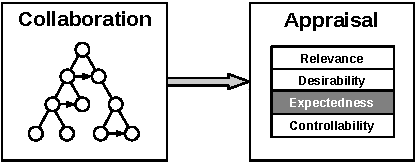
\includegraphics[width=0.4\textwidth]{figure/actionselection-croped.pdf}
  \vspace*{-3mm}
  \caption{{\fontsize{8}{9}\selectfont Influence of Collaboration on Appraisal
  (mechanisms in our framework).}}
  \label{fig:cpm}
  \vspace*{-6mm}
\end{figure}

The computational collaboration model in our work is strongly influenced by the
SharedPlans theory \cite{grosz:plans-discourse}. However, our algorithms are
also compatible with other collaboration theories, e.g., Joint Intentions theory
\cite{cohen:teamwork}. These theories have been extensively used to examine and
describe teamwork and collaboration. Yet, collaboration and emotion theories
have never been combined, as they are in our work. We believe a systematic
integration of collaboration theories and appraisal theory can help explain the
underlying processes of collaboration structure.

\begin{figure*}
  \centering
  \vspace*{-5mm}
  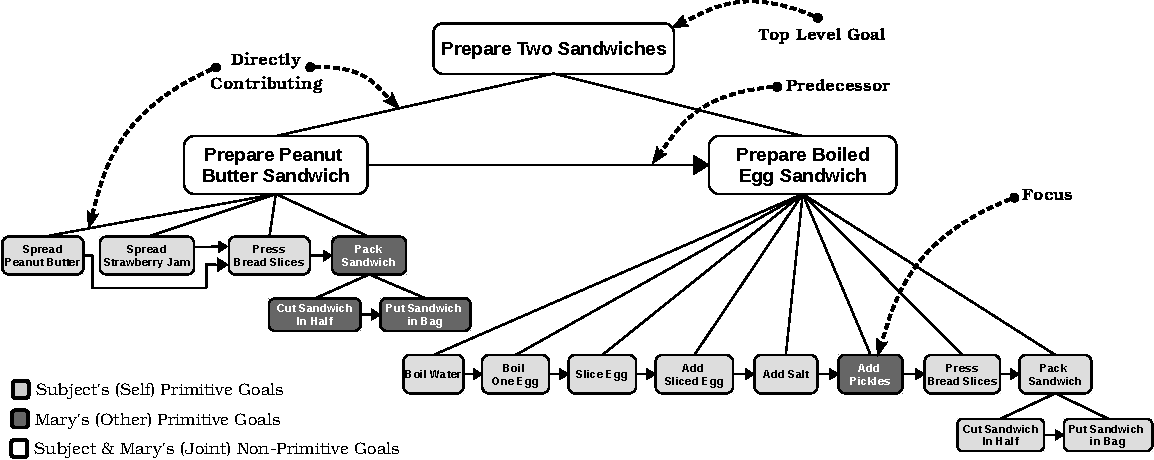
\includegraphics[width=14.5cm,height=5.225cm]{figure/taskModel-croped.pdf}
  \vspace*{-3mm}
  \caption{Example of collaboration structure (also used as task model for
  the evaluation).}
  \label{fig:taskModel}
  \vspace*{-3mm}
\end{figure*}

%Note that either {\textbf{.ps}} or {\textbf{.eps}} formats are
%used; use
%the \texttt{{\char'134}epsfig} or \texttt{{\char'134}psfig}
%commands as appropriate for the different file types.

\section{Collaboraiton}

The Collaboration mechanism constructs a hierarchy of goals associated with
tasks in a hierarchical task network (see Figure \ref{fig:taskModel}), and also
maintains the constraints and other required details of the collaboration
including the inputs and outputs of individual tasks, the preconditions
(specifying whether it is appropriate to perform a task), and the postconditions
(specifying whether a just-completed task was successful). Collaboration also
monitors the focus of attention, which determines the salient objects,
properties and relations at each point, and shifts the focus of attention during
the interaction.

\begin{itemize}[leftmargin=2pt]
  \setlength\itemsep{0.02mm}
  \item \textit{recognizeGoal($\varepsilon_t$)} returns the unique goal to which
  the given event (action, utterance, or emotional expression) directly
  contributes; it is only one goal since the robot can only do one primitive
  action at a time in our collaboration model, i.e, in the goal tree, a given
  primitive action can only directly contribute to one parent goal. The method
  returns \textit{ambiguous} if it does not recognize a goal in the
  plan\footnote{Ambiguity introduces some extra complexities which are beyond
  scope of this paper.}.
  
  \item \textit{getTopLevelGoal($g_t$)} returns $g_t$'s top level goal.
  
  \item \textit{isLive($g_t$)} returns \textit{true} if all the predecessors of
  $g_t$ are \textsc{achieved} and all the preconditions are \textsc{satisfied},
  i.e., \textsc{pending} or \textsc{in progress} goals; otherwise returns \textit{false}.
  
  \item \textit{isFocusShift($g_t$)} returns \textit{true} if the given
  goal is not the previous focus (top of the stack); otherwise returns
  \textit{false}.
  
  \item \textit{isNecessaryFocusShift($g_t$)} returns \textit{true} if the
  status of the previous focus was \textsc{achieved}; otherwise returns
  \textit{false} \cite{rich:focused-unfocused-users}.
  
  \item \textit{isPath($g_1$, $g_2$)} returns \textit{true} if there is a path
  between $g_1$ and $g_2$ in a plan tree structure; otherwise returns
  \textit{false}.
\end{itemize}

\section{Expectedness in Collaboraiton}

Expectedness is the extent to which the truth value of a state could have been
predicted from causal interpretation of an event
\cite{marsella:ema-process-model}. In the collaboration context the expectedness
of an event evaluates the congruency of the event with respect to the existing
knowledge about the shared goal. Thus, expectedness underlies a collaborative
robot's attention. Congruent beliefs in a robot's mental state will lead to more
consistent and effective outcomes of the processes in the overall architecture.
The collaboration mechanism uses expectedness to maintain the robot's attention
and subsequently its mental state with respect to the shared goal. Reciprocally,
the appraisal mechanism uses the underlying information of the collaboration
structure to evaluate the expectedness of an event. Therefore, a collaborative
robot uses expectedness to maintain its own mental state towards the shared
goal. The robot will also be able to respond to unexpected but relevant events.

\begin{algorithm}
	\caption{(Expectedness)}
	\label{alg:expectedness}
	\begin{algorithmic}[1]
		\Function{IsEventExpected}{Event $\varepsilon_t$}
			\Statex
			\State $\mathit{g}_{t} \gets \textit{recognizeGoal}{(\varepsilon_t)}$
			\State $\mathit{g}_{top} \gets \textit{getTopLevelGoal}{(\mathit{g}_{t})}$
			\Statex
			\If {$(\textit{isLive}{(\mathit{g}_{t})})$}
				\If {$(\neg \textit{isFocusShift}{(\mathit{g}_{t})}\hspace*{2mm}\OR$ \\
				\hspace*{13mm}$\textit{isNeccessaryFocusShift}{(\mathit{g}_{t})})$}
				\State \Return {\fontsize{7}{8}\selectfont MOST-EXPECTED}
				\Else
					\State \Return {\fontsize{7}{8}\selectfont EXPECTED}
				\EndIf
			\Else
				\If {$(\textit{isPath}{(\mathit{g}_{t}, \mathit{g}_{top})})$}
					\State \Return {\fontsize{7}{8}\selectfont UNEXPECTED}
				\Else
					\State \Return {\fontsize{7}{8}\selectfont MOST-UNEXPECTED}
				\EndIf
			\EndIf
		\EndFunction
	\end{algorithmic}
\end{algorithm}

In Algorithm \ref{alg:expectedness} we provide the process of computing the
expectedness based on the shared plan and status of the shared goal. The key
point in this algorithm is the status of the current shared goal
($\mathit{g}_{t}$) that is associated with the event $\varepsilon_t$ and its
relationship with the top level goal ($\mathit{g}_{_{top}}$).

The intuition captured here is that one expects the current goal to be finished
before undertaking another activity, but the goals that are the next focus of
attention are also to be expected \cite{rich:focused-unfocused-users}.
Therefore, if the goal is live, the algorithm checks whether the goal has not
changed, or the interpretation of the last event results in a necessary focus
shift. Shifting the focus to a new goal is necessary when the former goal is
achieved and a new goal is required. Consequently the new event is the
\textsc{most-expected} one. However, even if the focus shift is not necessary,
the new event can be considered as \textsc{expected}, since the corresponding
goal is already live. For goals that have not yet been started (that is, are not
live), the algorithm must determine how unexpected it would be to pursue one
now; if the goal is at least in the plan, i.e., on the path to the top level
goal, it is just \textsc{unexpected} while any others are
\textsc{most-unexpected}.

\section{Evaluation}

We conducted a user study to test our hypothesis that humans and our
expectedness algorithm will provide similar answers to questions related to
different factors used to compute expectedness. We conducted a between-subject
user study using an online crowdsourcing website --
CrowdFlower\footnote{http://www.crowdflower.com}. We had a questionnaire with 12
questions (including 2 test questions). There were originally 40 subjects. We
limited the subject pool to those with the highest confidence level on the
crowdsourcing website in the United States, Britain, and Australia. Test
questions were included to check the sanity of the answers. We eliminated
subjects providing wrong answers to our sanity questions, and subjects with
answering times less than 2 minutes.

To minimize the background knowledge necessary for our test subjects, we used a
simple example of preparing a peanut butter and jelly sandwich, and a hard
boiled egg sandwich. We provided textual and graphical instructions for the
questionnaire; Figure \ref{fig:taskModel} shows the corresponding task
model. The instructions presented a sequence of hypothetical collaborative tasks
to be carried out by the test subject and an imaginary friend, Mary. We also
provided a simple definition for expectedness appraisal variable. The questions
introduced specific situations related to the shared plan, which included
blocked tasks and failure or achievement of a shared goal. Each question
provided three answers which were counterbalanced in the questionnaire. We
provided an option like C in all questions, because we did not want to force
subjects to choose between two options when they did not have a good reason.
There were two questions designed based on each factor that we use in our
algorithm. The questions were randomly placed in the questionnaire. Figure
\ref{fig:qs1} shows an example question from the questionnaire. The input for
our algorithms was the task model depicted in Figure \ref{fig:taskModel}.

\begin{figure}[tbh]
  \vspace{-1mm}
  \centering
  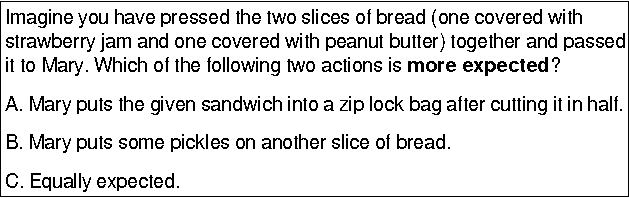
\includegraphics[width=0.48\textwidth]{figure/question-sample-croped.pdf}
  \vspace*{-7mm}
  \caption{{\fontsize{9}{9}\selectfont Example Expectedness Question.}}
  \label{fig:qs1}
  \vspace{-2mm}
\end{figure}

Average results and standard deviation of the fractions of subjects' answers
agreeing with our algorithm output was 0.785 and 0.120 respectively. Each
question had 3 answers. Therefore, a random distribution would result in 33\%
agreement with our algorithm's output. However, the average agreement between
our algorithm and the human subjects was 78.5\%. Our results indicate that
people largely performed as our hypothesis predicted. The \textit{p}-value
obtained based on a one-tailed z-test shows the probability of human subjects'
answers being generated from a random set. The very small \textit{p}-value
(<0.001) indicates that the data set is not random; in fact, the high percentage
of similarity confirms our hypothesis and shows that the algorithm can help us
to model expectedness as an appraisal in collaboration.

\section{Conclusion}
The SharedPlans theory and other computational collaboration theories (e.g.,
Joint Intentions) emphasize the importance of commitment in collaboration.
According to these theories collaborators are required to commit to their shared
plan or intentions to successfully collaborate and achieve a shared goal. This
commitment requires them to appraise their environment based on the shared plan
structure. In our next step, we want to test our appraisal algorithms and their
influence on action selection during collaboration. This study will be conducted
between a KUKA youbot and human subjects on a different task model.

\section*{Acknowledgments}

{\fontsize{8.2}{9}\selectfont This work is supported by the National Science
Foundation under award IIS-1012083.}

\bibliographystyle{abbrv}
\bibliography{mshayganfar}

\end{document}